
\section{符号坐标与用户变换}

\PGFPlots{} 支持可应用于输入和输出坐标的用户变换。假设图要显示随时间变化的天数与账户对账单。那么，人们想可视化日期与信贷余额。但是：在此之前日期需要变换为数字！此外，刻度标签也应显示为日期。这种以及更一般的变换，可以使用 |x coord trafo| 和 |y coord trafo| 键来实现。


\paragraph{备注：}

本节适用于想要非标准输入\emph{坐标}的用户。如果你有不需要变换的普通数字，并且希望刻度标签使用特殊符号，应考虑使用第~\pageref{pgfplots:key:xticklabels} 页描述的 |xticklabels|（|yticklabels|）键。

有关不同类型的变换及其相互作用，另请参见 Section~\ref{sec:transformation:interaction}。

\begin{pgfplotsxycodekeylist}{%
    \x\ coord trafo,
    \x\ coord inv trafo%
}
    这些代码键允许任意坐标变换，应用于输入坐标和输出刻度标签。

    |x coord trafo| 和 |y coord trafo| 命令键接受一个参数，即输入坐标。它们应将 |\pgfmathresult| 设置为最终值。

    在这个层面，输入坐标按其在 |\addplot| 语句中的原样提供。例如，如果 $x$ 坐标实际上是 \meta{year}-\meta{month}-\meta{day} 形式，例如 |2008-01-05|，那么一个有用的坐标变换会将此字符串变换为数字（预定义实现见下文）。

    简而言之，应用此变换时\emph{尚未}对输入坐标应用任何数值处理。\footnote{当然，如果坐标是由 gnuplot 或 \pgfname{} 生成的，则不再成立。}

    输入坐标变换应用于
    %
    \begin{itemize}
        \item 任何输入坐标（用 |\addplot| 或 |axis cs| 指定），
        \item 任何用户指定的 |xtick| 或 |ytick| 选项，
        \item 任何用户指定的 |extra x ticks| 和 |extra y ticks| 选项，
        \item 任何用户指定的坐标轴界限，如 |xmin| 和 |xmax|。
    \end{itemize}

    输出坐标变换 |x coord inv trafo| 在求值 |xticklabel| 和 |yticklabel| 键之前应用于刻度位置。|x coord inv trafo| 的参数是一个定点数（小数点后可能有尾随零）。刻度标签代码可以使用逆变换定义的附加宏。

    备注：\PGFPlots{} 将照常生成刻度位置，不应用额外技巧。如果默认值不能正确遵守坐标空间，可能需要显式提供刻度位置。

    这些键的初始值为
    %
\begin{codeexample}[code only]
\pgfplotsset{
    x coord trafo/.code={},
    x coord inv trafo/.code={},
}
\end{codeexample}
    %
    \noindent 它简单地禁用变换（$y$ 当然也一样）。


    \paragraph{备注：}

    可能需要设置
    %
\begin{codeexample}[code only]
\pgfplotsset{
    xticklabel={\tick},
    scaled x ticks=false,
    plot coordinates/math parser=false,
}
\end{codeexample}
    %
    \noindent 以避免对 |\tick| 进行数字格式化例程或对刻度缩放方法进行数值处理。这由预定义的符号坐标样式自动完成（见下文）。
\end{pgfplotsxycodekeylist}


\subsection{字符串符号作为输入坐标}

可以向 \PGFPlots{} 提供一个字符串字典。然后输入坐标可以使用该字典中提供的任何符号。

\begin{pgfplotsxykeylist}{symbolic \x\space coords=\marg{dictionary}}
    一个设置 |x coord trafo| 和 |x coord inv trafo|（或相应的 |y| 或 |z| 变体）的样式，使 \meta{dictionary} 中的任何元素都是有效的输入坐标。\meta{dictionary} 可以是逗号分隔列表或以 `|\\|' 结尾的列表。在两种情况下，空白都被视为名称的一部分（在行尾使用 `|%|'）。

    字典会为每个元素分配整数（从 $0$ 开始）。这些整数在内部用于算术。最后，逆变换接受一个定点数并将其映射到最近的整数，然后该整数映射到字典中。
    %
\begin{codeexample}[]
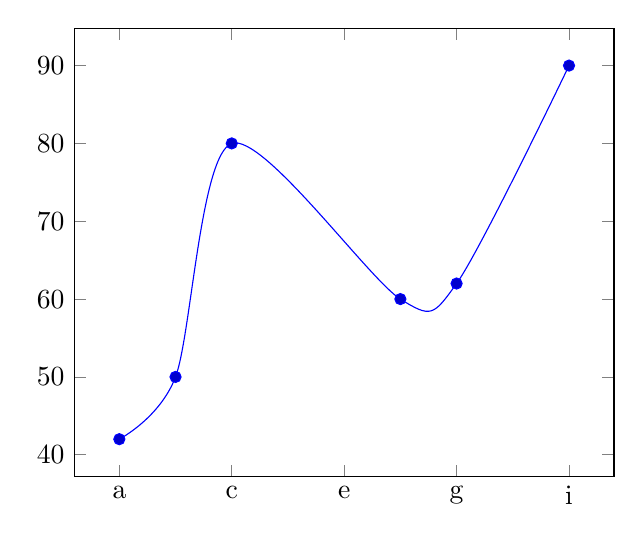
\begin{tikzpicture}
\begin{axis}[
    symbolic x coords={a,b,c,d,e,f,g,h,i},
]
    \addplot+ [smooth] coordinates {
        (a,42)
        (b,50)
        (c,80)
        (f,60)
        (g,62)
        (i,90)
    };
\end{axis}
\end{tikzpicture}
\end{codeexample}

    该变换的效果仅仅是输入坐标可以是字典的元素，刻度标签也将从该字典中选择。

    请注意，|symbolic x coords| 或多或少等价于显式提供的 |xtick| 位置和 |xticklabels|：
    %
\begin{codeexample}[]
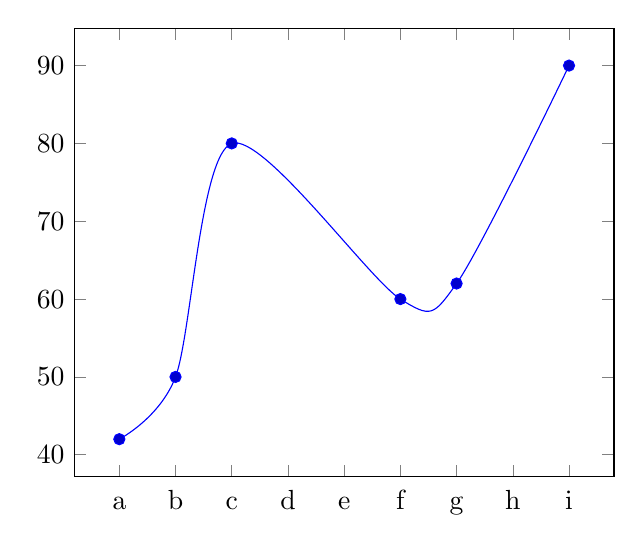
\begin{tikzpicture}
\begin{axis}[
    xtick={0,1,2,...,20},
    xticklabels={a,b,c,d,e,f,g,h,i},
    xticklabel style={
        anchor=base,
        yshift=-\baselineskip,
    },
]
    \addplot+ [smooth] coordinates {
        (0,42)
        (1,50)
        (2,80)
        (5,60)
        (6,62)
        (8,90)
    };
\end{axis}
\end{tikzpicture}
\end{codeexample}
    %
    \noindent 区别在于，使用 |symbolic x coords| 的方法更易读，而 |xtick| 方法在坐标算术方面更简单（例如使用 |enlargelimits| 增大界限）。这里的 |xticklabel style| 是尝试将所有刻度标签对齐到其基线（一旦标签有超出基线的字符，这对 |symbolic x coords| 也有用）。

    键 |symbolic x coords| 及其变体接受逗号分隔的字符串列表。这些可以是任意的，甚至可以包含不可展开的材料：\footnote{自 \PGFPlots{} 1.11 版起。}
    %
\begin{codeexample}[]
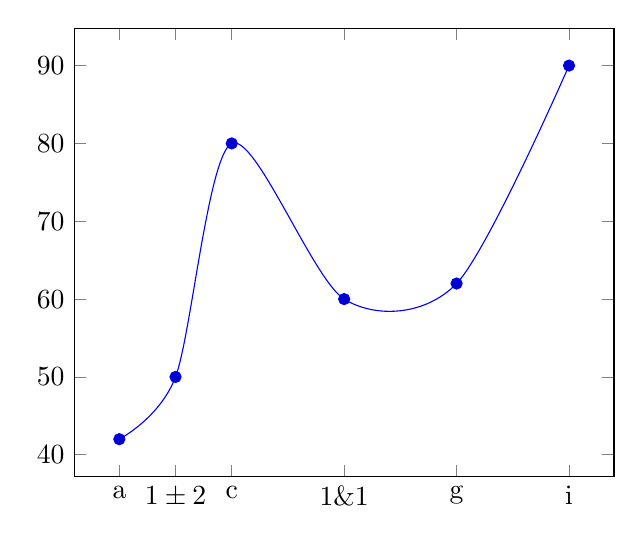
\begin{tikzpicture}
\begin{axis}[
    symbolic x coords={a,$1 \pm 2$,c,d,1\&1,f,g,h,i},
    xtick=data,
]
    \addplot+ [smooth] coordinates {
        (a,42)
        ($1 \pm 2$,50)
        (c,80)
        (1\&1,60)
        (g,62)
        (i,90)
    };
\end{axis}
\end{tikzpicture}
\end{codeexample}
    %
    在任何情况下，都必须精确匹配 \meta{dictionary} 的参数，包括任何空白。

    符号坐标很有用，因为它们减少了将字符串映射到索引（反之亦然）的负担。然而，它们有一个注意事项：如果你想将 |xmin| 设置为第一个 |symbolic x coord| 左侧的值怎么办？这是不可能的，因为任何输入坐标都应包含在 |symbolic x coord| 中。为了仍然允许此类修改，\PGFPlots{} 会检查神奇前缀 \index{Symbolic coords![normalized]}\declareandlabel{[normalized]}：
    %
\begin{codeexample}[]
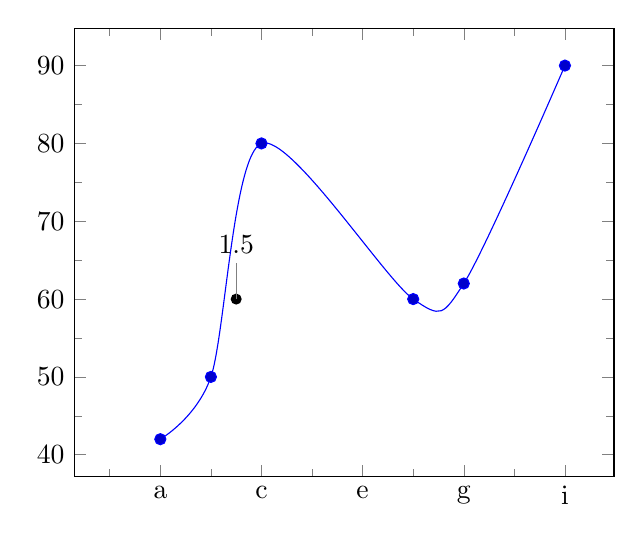
\begin{tikzpicture}
\begin{axis}[
    symbolic x coords={a,b,c,d,e,f,g,h,i},
    xmin={[normalized]-1.7},
    minor tick num=1,
]
    \addplot+ [smooth] coordinates {
        (a,42)
        (b,50)
        (c,80)
        (f,60)
        (g,62)
        (i,90)};

    \fill (axis cs:{[normalized]1.5},60)
        circle (2pt) coordinate [pin={$1.5$}];
\end{axis}
\end{tikzpicture}
\end{codeexample}
    %
    每当 \PGFPlots{} 找到一个以精确字符串 `|[normalized]|' 开头的符号坐标时，它会将该前缀之后的所有内容解释为规范化数字，而\emph{不是}符号。在我们的示例中，|xmin| 将设置为 $-1.7$，即 $a$ 左侧的值（根据上面的定义，$a$ 为 $0$）。此外，自定义 |\node| 放置在 $(1.5,60)$，尽管 $1.5$ 不是定义的符号——但我们知道它在 |b| 和 |c| 之间，它们分别是字典条目 $1$ 和 $2$。


    \paragraph{另请参阅}

    使用 |xtick=data|（或 |minor xtick=data|）在每个遇到的坐标处添加刻度和/或网格线的选项。
\end{pgfplotsxykeylist}


\subsection{日期作为输入坐标}
\label{sec:pgfplots:date:coords}

{
\def\pgfplotsmanualcurlibrary{dateplot}

前面提到的使用日期作为输入坐标的应用已被预定义，并支持小时和分钟。它依赖于 \pgfname{} 日历库，该库将日期转换为儒略历中的数字。然后，一个坐标单位为一天。

\begin{pgfplotslibrary}{dateplot}
    加载坐标变换代码。
\end{pgfplotslibrary}

\begin{stylekey}{/pgfplots/date coordinates in=\meta{coordinate}}
    安装 |x coord trafo| 和 |x coord inv trafo|（或 \meta{coordinate} 的相应变体），使 \meta{year}|-|\meta{month}|-|\meta{day} 形式的 ISO 日期被接受。这里，\meta{coordinate} 通常是 |x|、|y| 或 |z| 之一，但它也可以包含类似 |hist/data| 的内容。

    安装此样式后，像 |2006-02-28| 这样的输入值将使用儒略历转换为“适当的”整数。输入坐标可以是以下形式

        \meta{year}|-|\meta{month}|-|\meta{day}

    \noindent 或者它们可以包含时间，如

        \meta{year}|-|\meta{month}|-|\meta{day} \meta{hour}|:|\meta{minute}.

    变换的结果是数字，其中一个单位为一天，时间为分数。

    该变换使用 \pgfname-calendar 模块实现，参见 \cite[Calendar Library]{tikz}。该参考还包含有关日期扩展语法选项的更多信息。

    逆变换提供以下宏，它们在刻度标签求值期间可用（即在 |xticklabel| 或 |yticklabel| 内部使用时）：
    %
    \begin{itemize}
        \item \declareandlabel{\year} 展开为年分量，
        \item \declareandlabel{\month} 展开为月分量，
        \item \declareandlabel{\day} 展开为日分量，
        \item \declareandlabel{\hour} 展开为小时分量（使用两位数字），
        \item \declareandlabel{\Hour} 展开为小时分量（但省略前导零），
        \item \declareandlabel{\minute} 展开为分钟分量（两位数字），
        \item \declareandlabel{\Minute} 展开为分钟分量（省略前导零），
        \item \declareandlabel{\lowlevel} 展开为表示该刻度的底层数字，
        \item \declareandlabel{\second} 始终为 |00|。
    \end{itemize}
    %
    例如，这允许在 |xticklabel| 内部使用 |\day.\month.\year| 或 |\day. \hour:\minute|。

    下面展示一个完整示例（使用虚构数据）。
    %
\pgfplotsset{anchor=center,/tikz/every picture/.append style={baseline}}
% \usepgfplotslibrary{dateplot}\usepackage{eurosym}
\begin{codeexample}[]
% requires \usepgfplotslibrary{dateplot} !

\pgfplotstabletypeset[string type]{plotdata/accounts.dat}

\begin{tikzpicture}
    \begin{axis}[
        date coordinates in=x,
        xticklabel={\day.\month.},
        xlabel={2008},
        stack plots=y,
        yticklabel={\pgfmathprintnumber{\tick}\EUR{}}, % <- requires \usepackage{eurosym}
        ylabel=Total credit,
        ylabel style={yshift=10pt},
        legend style={
            at={(0.5,-0.3)},anchor=north,legend columns=-1,
        },
    ]
        \addplot table [x=date,y=account1] {plotdata/accounts.dat};
        \addplot table [x=date,y=account2] {plotdata/accounts.dat};
        \addplot table [x=date,y=account3] {plotdata/accounts.dat};
        \legend{Giro,Tagesgeld,Sparbuch}
    \end{axis}
\end{tikzpicture}
\end{codeexample}

% \usepgfplotslibrary{dateplot}\usepackage{eurosym}
\begin{codeexample}[]
% requires \usepgfplotslibrary{dateplot} !
\begin{tikzpicture}
\begin{axis}[
    date coordinates in=x,
    xtick=data,
    xticklabel style=
        {rotate=90,anchor=near xticklabel},
    xticklabel=\day. \hour:\minute,
]
    \addplot coordinates {
        (2009-08-18 09:00,  050)
        (2009-08-18 12:00,  100)
        (2009-08-18 15:00,  100)
        (2009-08-18 18:35,  100)
        (2009-08-18 21:30,  040)
        (2009-08-19,        020)
        (2009-08-19 3:00,   000)
        (2009-08-19 6:0,    035)
    };
\end{axis}
\end{tikzpicture}
\end{codeexample}
\end{stylekey}

\begin{pgfplotskey}{date ZERO=\meta{year}-\meta{month}-\meta{day}}
    一个技术键，用于定义 |date coordinates in| 的 $0$ 坐标。

    直到并包括 1.12 版本的 \PGFPlots{} 需要此值。自 1.13 版起，第一个遇到的坐标被用作 |date ZERO|，即它在没有用户干预的情况下自动分配。

    用户永远不会看到生成的数字，因此可能永远不需要更改此值。此键允许根据需要设置结果。
\end{pgfplotskey}

}
